\section{Summary}
\label{sec:conclusions}

Measurements of the inclusive $\Wo$ and $\Zo$ production cross sections have been performed 
using a data sample of pp collision events at $\sqrt{s}=7\TeV$ 
collected with the CMS detector at the LHC in 2010 and 
corresponding to an integrated luminosity of 36~pb$^{-1}$. 
The inclusive production cross sections of $\Wp$ and $\Wm$ have been measured separately 
as well as the ratios of the $\Wp/\Wm$ and $\Wo/\Zo$ production cross sections.  
All measurements are dominated by systematic uncertainties,  
the main uncertainty originating from the integrated luminosity (4\%), which cancels in the ratios.
Experimental systematic uncertainties range from
0.7 to 1.8\%, and theoretical uncertainties range from 0.9 to 2.1\%.
The measurement of the $\Wo/\Zo$ cross-section ratio also leads to an
indirect determination of $\Gamma(\Wo)$, which is in agreement with the
current world average. 
%and with the SM prediction.

The results agree with the ATLAS measurement~\cite{WZATLAS:2010} 
and with previous CMS results~\cite{WZCMS:2010}.
All measurements are consistent with the SM NNLO predictions.



%Figure~\ref{fig:WZsigmas} shows the CMS W and Z cross section measurements together 
%with measurements at lower center-of-mass energy hadron colliders.
%The predicted increase of the cross sections with center of mass energy is confirmed
%by our measurements. 
%
%
% \begin{figure}
% \begin{center}
% 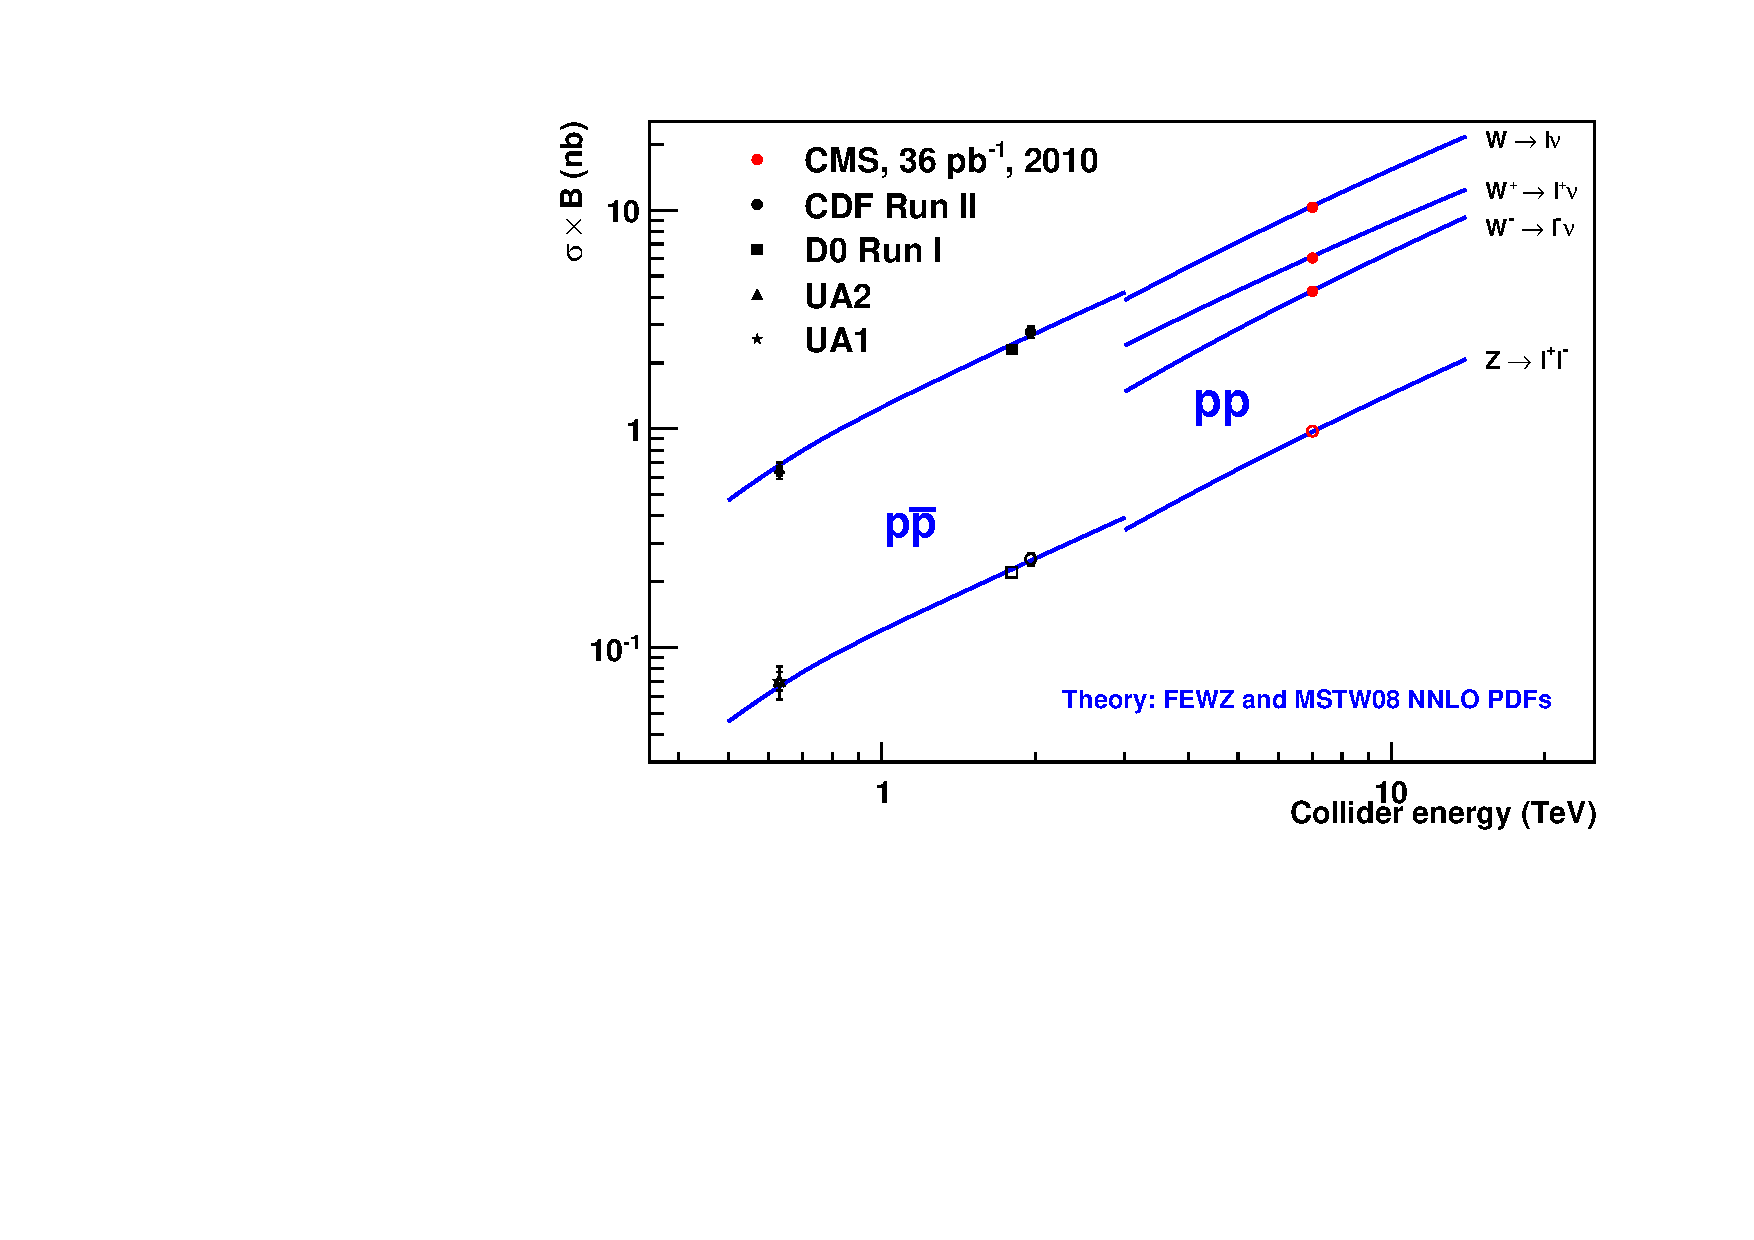
\includegraphics[width=0.8\textwidth]{figs/WZsigmas.pdf}
% %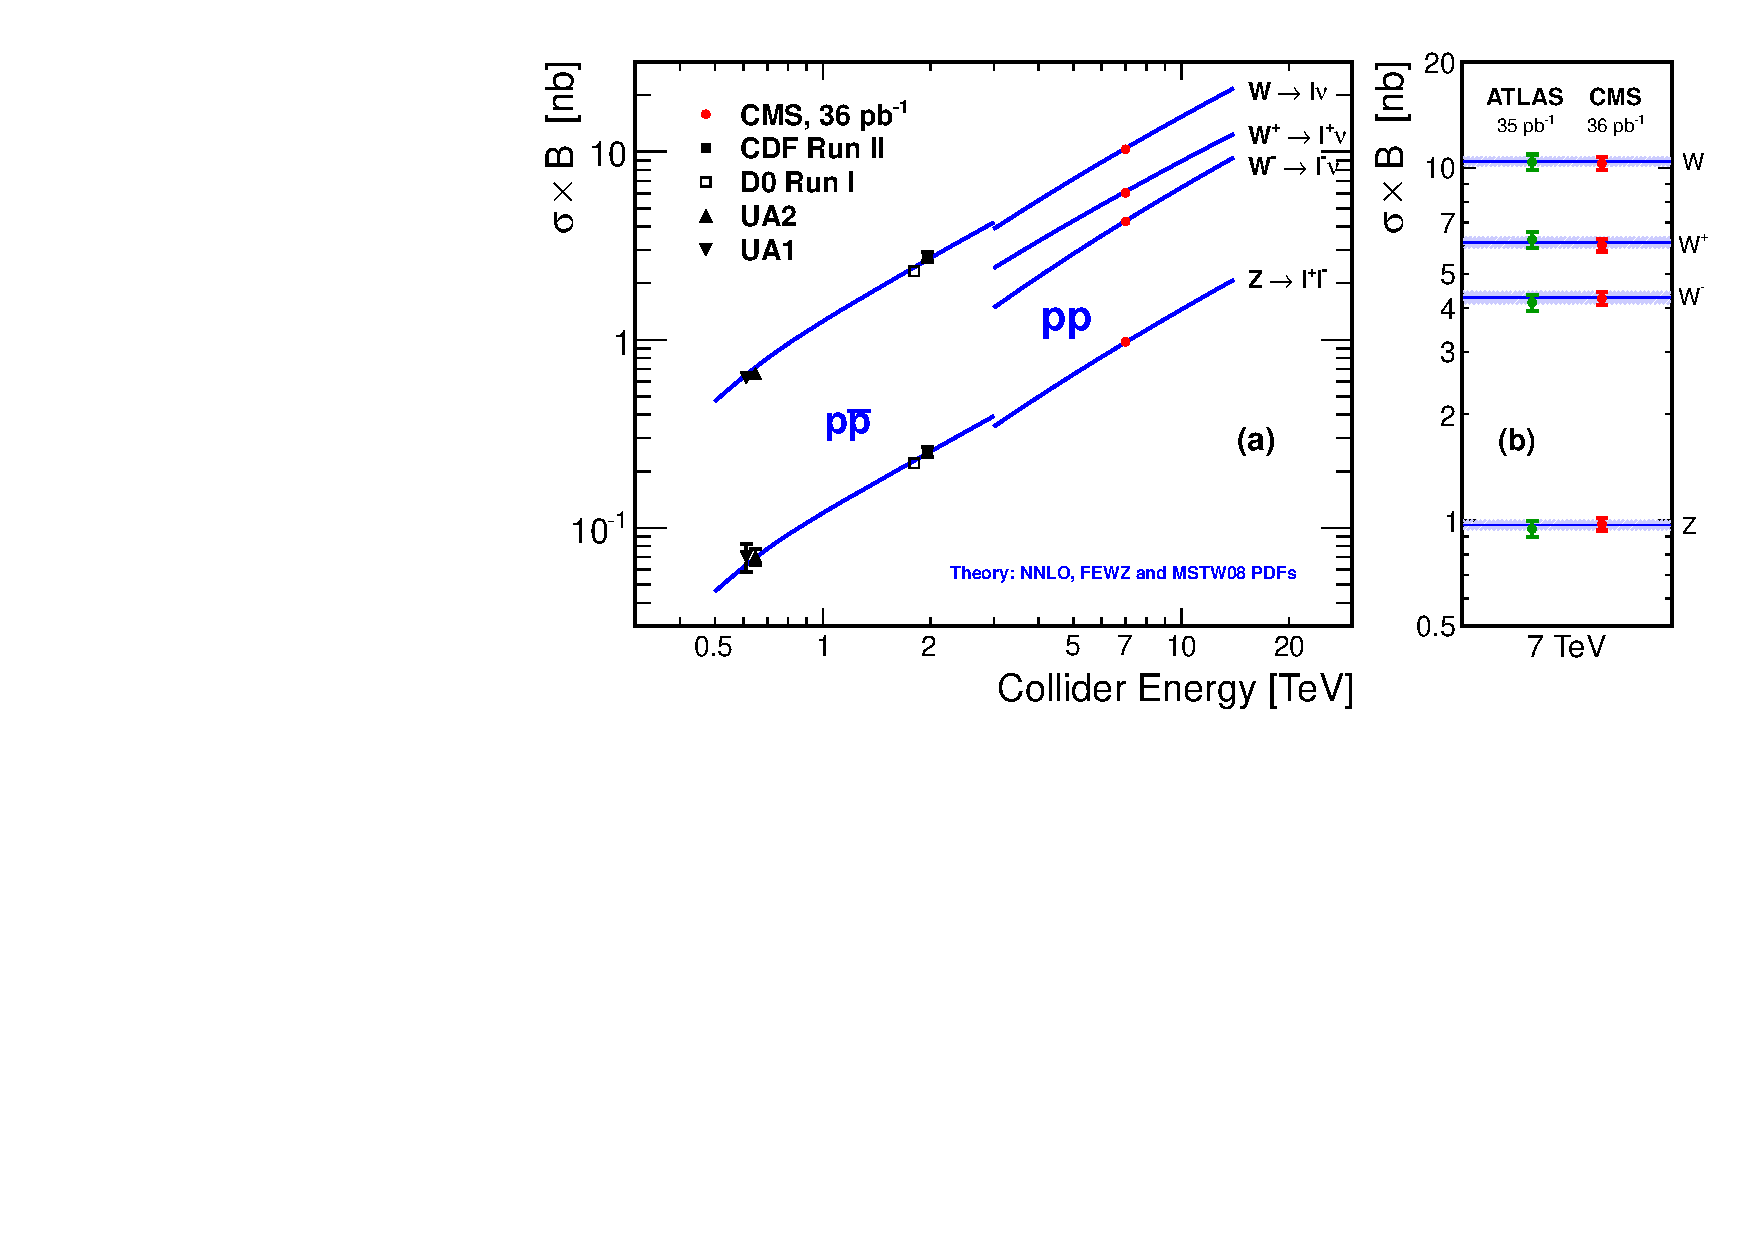
\includegraphics[width=1\textwidth]{figs/atlas-cms.pdf}
% \caption[.]{\label{fig:WZsigmas}
% Measurements of inclusive W and Z production cross sections 
% times branching ratios as a function of center-of-mass energy for CMS and experiments
% at lower-energy colliders. The lines are the NNLO theory predictions.
% %The solid symbols represent
% %$\sigma( \pp \to \Wo X)\times {\cal B}(\Wo\rightarrow\ell\nu)$ and the
% %hollow symbols, $\sigma(\pp\to\Zo X)\times {\cal B}(\Zo\rightarrow\ell^+\ell^-)$.
% %Theoretical predictions are shown as blue lines.
% %(b) A comparison with the latest preliminary ATLAS results with 35~pb$^{-1}$ from Ref.~\cite{WZATLAS:2011}
% %is shown. The blue lines show the theoretical predictions with their uncertainty.
% %CMS (red, four points on the right side) and ATLAS (green, four point on the left side) measurements are shown with the total experimental, theoretical
% %and luminosity uncertainties. The luminosity uncertainties amount to 3.4\% for ATLAS and 4\% for CMS.
% }
% \end{center}
% \end{figure}


